\section{Aufbau der Stoffe} {SW 1-2 ~}

\subsection{PSE - Periodensystem}
\begin{center}
	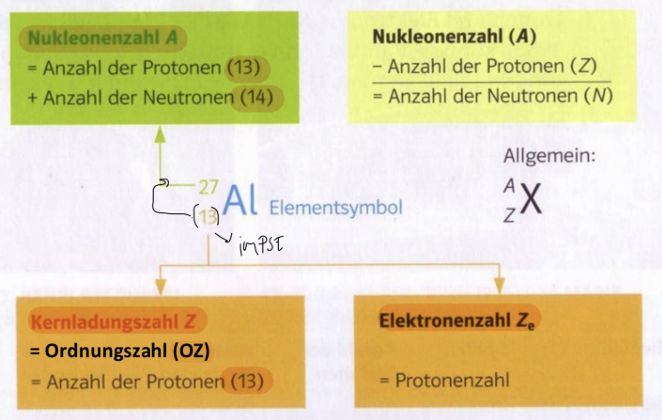
\includegraphics[height=3cm]{images/Nukleonenzahl.jpg}
\end{center}

\begin{tabular} {l}
	- Protonen und Neutronen sind sog. Nukleonen, \\
	sie wird oftmals auch Massenzahl bezeichnet. \\
\end{tabular}

\subsection{Stoffe}	
\renewcommand{\arraystretch}{1.2}
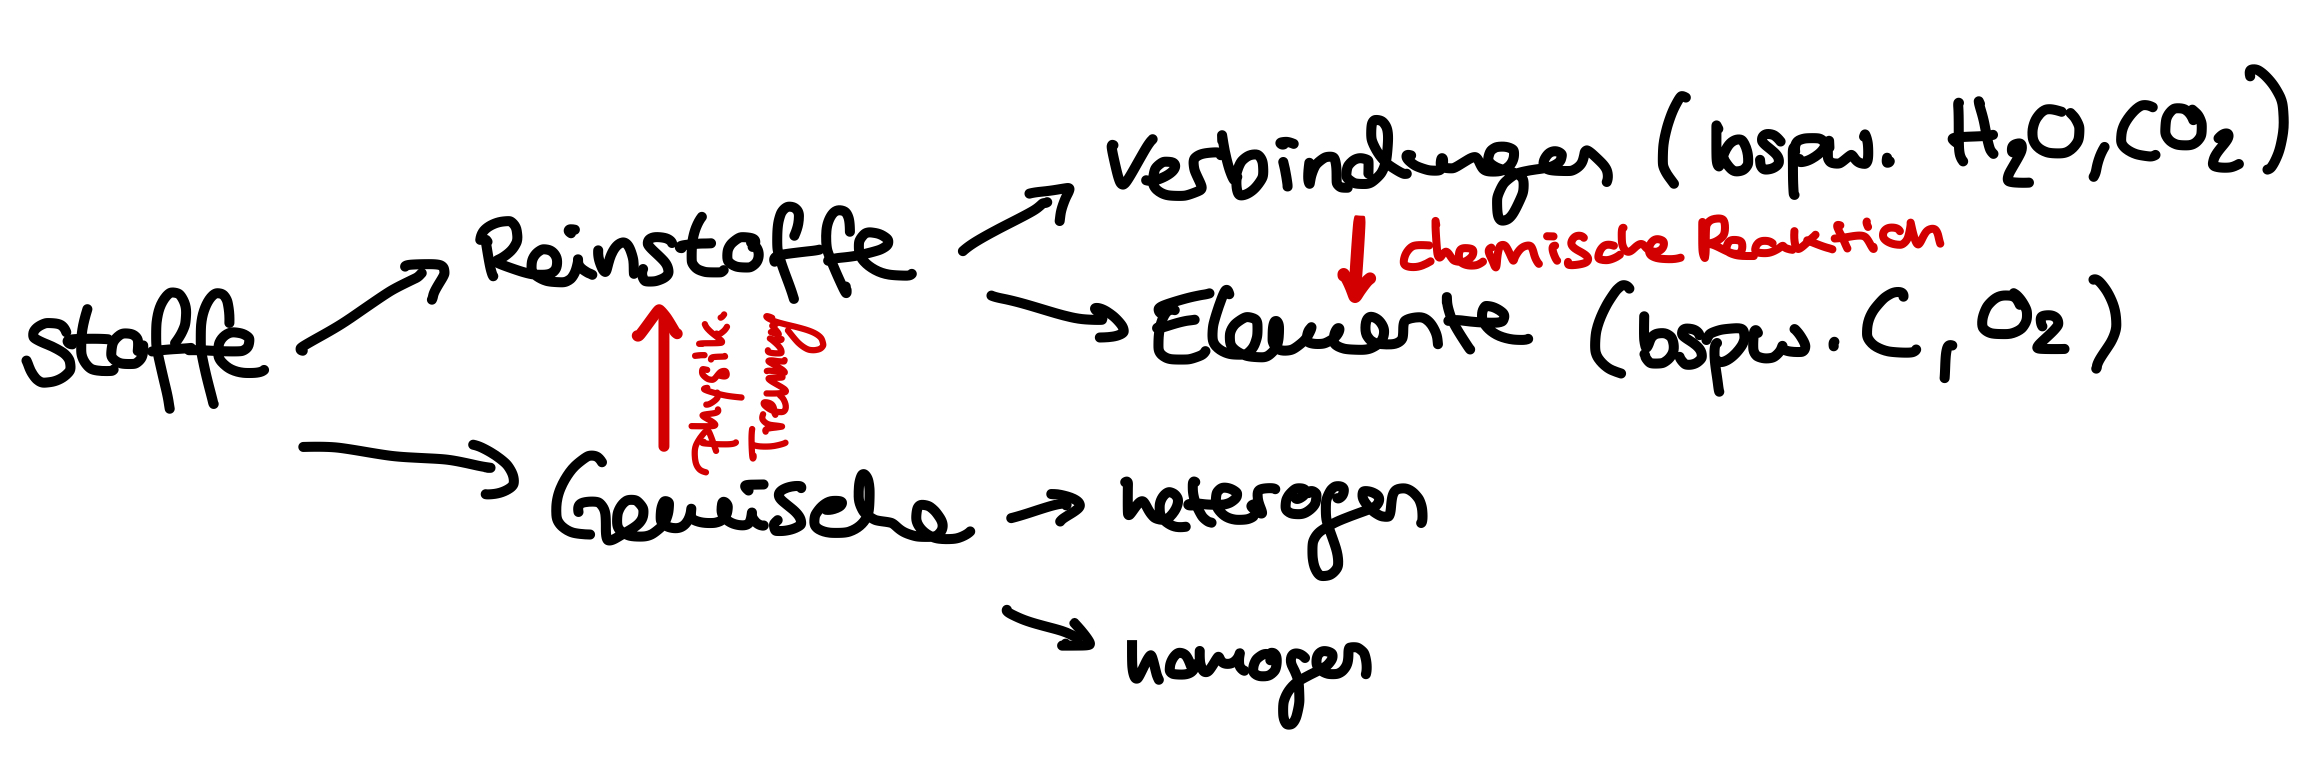
\includegraphics[width=\columnwidth]{images/Stoffe_eigenschaften.PNG}

\subsection{Aggregatzustand}		

{\footnotesize
	\begin{tabular}[\columnwidth]{l l | l l}
			\underline{\textbf{Aggregatzustand}} 	&     					& \underline{\textbf{Dispersitätsgrad}}    &   \\ 
			\textbf{Dispersionsmittel}  	& \textbf{Dispergierter Stoff}	& \textbf{Heterogen}   		& \textbf{Homogen}       \\
			gasförmig (g) 		& gasförmig (g)        	& -          		& Gasgemisch        \\
			gasförmig (g)		& flüssig (l)			& Nebel				& -		\\
			gasförmig (g)		& fest (s)				& Rauch				& -		\\
			flüssig (l)			& gasförmig (g) 		& wenig haltbarer Schaum	& Gaslösung		\\
			flüssig (l)			& flüssig (l) 			& wenig haltbare Emulsion				& Flüssigkeitslösung		\\
			flüssig (l)			& fest (s) 				& Suspension				& feststofflösung	\\
			fest (s)			& gasförmig (g) 		& fester Schaum* 			& 		\\
			fest (s)			& flüssig (l) 			& brei				&		\\
			fest (s)			& fest (s) 				& Feststoffgemische				& legierung zweier Metalle	\\
			*( zB. Schaumstoff) 	&				&						& \\
	\end{tabular} 
}
		
\subsection{Eselsbrücke}

\begin{tabular}{ll} 
	\textbf{HONClBrIF – "der Brief vom Onkel"}   &  Die Buchstaben stellen dabei \\
	& die Elemente des PSE dar, die in der \\
	& Natur nur 2-atomig vorkommen. \\ & \\
	Ausnahme: & $P_4$ (Phosphor) und $S_8$ (Schwefel)  \\
\end{tabular}
\renewcommand{\arraystretch}{1}  

\subsection{Kugelwolkenmodell}	
\begin{center}
	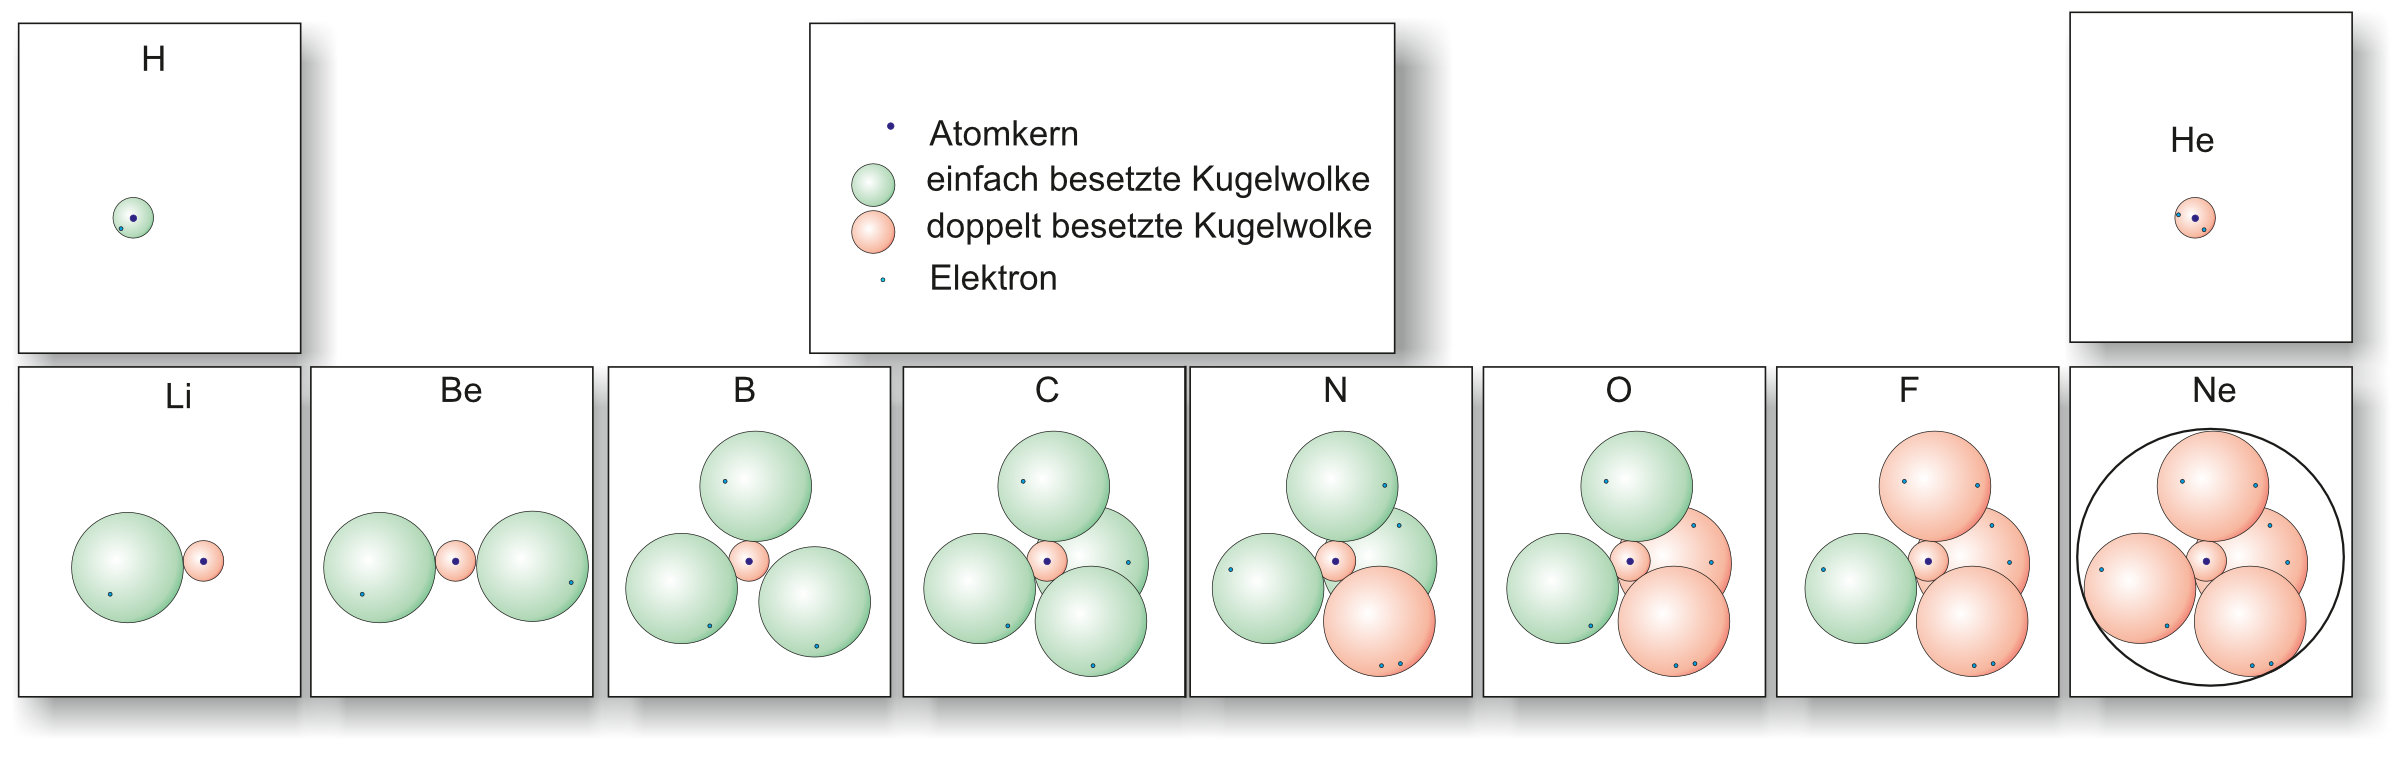
\includegraphics[width=\columnwidth]{images/kugelwolkenmodell.jpg}
\end{center}

\subsection{Bindungswinkel}
\begin{center}
	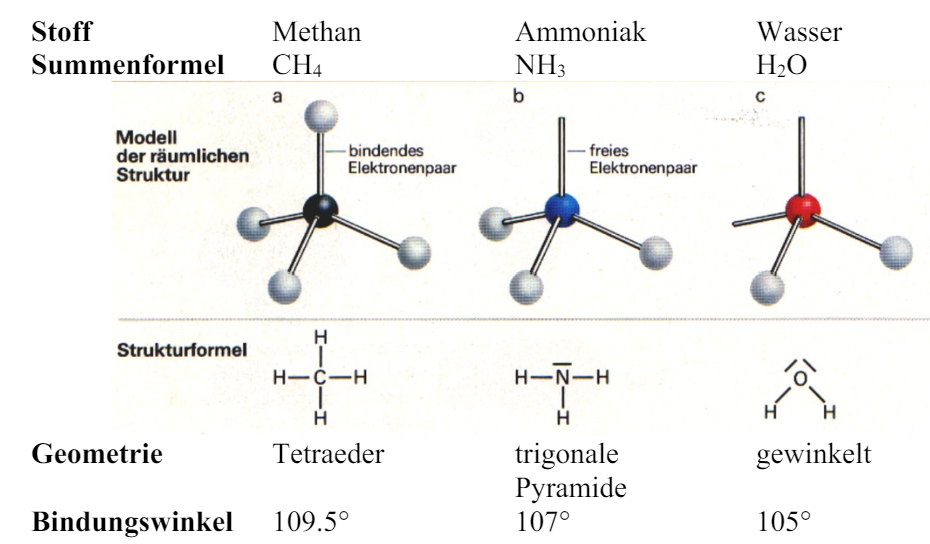
\includegraphics[height=4cm]{images/Winkel.png}
\end{center}

\subsection{Schreibweisen von Lewis} 

\begin{center}
	\includegraphics[width=\columnwidth]{images/lewis-schreibweise.png}
\end{center}
\begin{center}
	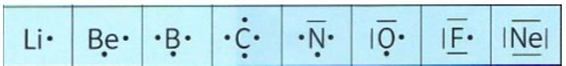
\includegraphics[width=\columnwidth]{images/Lewis-schreibweise_2.png}
\end{center}

\begin{tabular}{l}
	Anzahl anhand der \textbf{Hauptgruppen (1-8)}~ im PSE bestimmbar \\
	\\
	\textbf{Beispiel}: \\
	Natrium (Na): 1. Hauptgruppe = 1 Ve \\
	Kohlenstoff (C): 4. Hauptgruppe = 4 Ve \\
	\\
	Bestimmung der \textbf{Nebengruppen} komplizierter/unmöglich \\ -> nicht Prüfungsrelevant \\
\end{tabular}


\subsection{Isotope}
\begin{tabular}{l}
	\textbf{Isotope} sind Nuklide (=gleichen Atomsorte) mit der gleichen Ordnungszahl \\ (=Protonen),
	\textbf{aber unterscheiden sich von der Anzahl Neutronen}. \\ 
	Die meisten \underline{natürlichen Elemente haben ein oder paar stabile Isotope,} \\
	während andere Isotope vom gleichen Element \underline{radioaktiv} sind (=instabil). \\ Dann spricht man von $\alpha , \beta , \gamma -Zerfall$ . \\

\end{tabular}
  
           